\chapter{\Dappcoder{}: A Decentralized Marketplace for dApp Crowdsourcing}
\label{chapter:devid}

\emph{Decentralized applications, also known as dApps, are the new paradigm for writing business-critical software.
Crowdsourcing the development of such applications is gaining popularity.
At the same time, finding developers with appropriate qualifications and skills for this activity is key, yet challenging.
The main problem is that the portfolio of developers is usually scattered across centralized crowdsourcing platforms, and vendor locked.
This can result in an incomplete impression of their capabilities.}

\emph{In this chapter we address these problems and first introduce a unified, blockchain-based portfolio for developers, named \emph{DevID}.
Over time, a DevID portfolio enables developers to build up a trustworthy collection of records that showcase their capabilities and expertise.
They can import data assets from third parties into their portfolio, add projects and skills, and receive endorsements from others.
All portfolio records are stored on an existing, scalable ledger, named TrustChain, and managed by developers themselves.
TrustChain enables tamper-proof data accounting with low overhead and without network-wide consensus.}

\emph{We then build a decentralized crowdsourcing marketplace, named \emph{dAppCoder}, for the development of dApps.
dAppCoder allows clients to publish projects and developers can find work, all without trusted intermediaries.
dAppCoder utilizes DevID portfolios to match these clients and developers.
We fully implement DevID and dAppCoder and conduct a deployment trial.
Our trial demonstrates that DevID is efficient at storing portfolio records. }

\newpage

\section{Introduction}
\label{sec:introduction}
Decentralized applications, also known as dApps, allow for contractual logic that runs without the need for trusted intermediaries~\cite{raval2016decentralized}.
At the time of writing, there are thousands of decentralized applications deployed on numerous blockchain solutions, most of which are on Ethereum.
The dApp ecosystem is continuously expanding and recently has been accelerated by the rise of decentralized finance (DeFi) solutions~\cite{zetzsche2020decentralized}.

Since dApps usually require a high level of security and robustness, the engineering of dApps is considered a challenging task and there is a shortage of talent capable of building these solutions~\cite{shortage2016nasdaq}.
For this reason, crowdsourcing the development of decentralized applications is becoming an increasingly popular alternative to training in-house talent~\cite{gong2021reference}.
Crowdsourcing is a relatively new model for software development, where an open call is made for the documentation, design, coding, and testing of software~\cite{latoza2016crowdsourcing}.
Match clients and developers is at the core of numerous intermediary crowdsourcing markets such as Upwork and Fiverr.
These profit-driven markets usually charging a commission of all payments between a client and a developer.

Unfortunately, existing crowdsourcing platforms only provides access to a subset of all available work and developers.
%Therefore, finding the right talent to develop decentralized applications across different platforms can be challenging and time-consuming.
Specifically, the key problem is that centralized market approaches for client-developer matching lead to \emph{fragmentation} and \emph{lock-in} effects~\cite{pouwelse2017laws,gong2021reference}.
Many software developers have their portfolios and programming activities fragmented across multiple platforms, like TopCoder, GitHub and LinkedIn.
Each platform only yields a partial impression on the capabilities and background of a developer, making it challenging for a client to make an educated decision on who to hire for a particular task.
Additionally, data assets are usually locked to one platform and cannot easily be exported across different services, complicating this matchmaking process even more~\cite{hesse2019reputation}.

%Another issue associated with centralized approaches is \emph{data authority}.
%It raises much discussion in our society, where data-driven corporates control the vast majority of our personal data.
%By agreeing to the terms of service of a company, one essentially gives them authority over most of the personal data being shared.

There currently is no independent platform for dApp crowdsourcing without fragmentation and lock-in effects.
We argue that the availability of such a platform would increase efficiency and effectiveness when matching reputable developers looking for work and clients that are in need of talent.
In other words, such a platform would reduce \emph{search frictions}, which are impediments to finding matches between clients and developers.
In this work, we address this deficiency.
As a first step, we design \emph{DevID}, a unified portfolio for software developers.
We believe that such a portfolio is a key precursor to a more efficient crowdsourcing marketplace, since highlighting the expertise of a developer is a key step in the client-developer matchmaking process.
DevID portfolios enable developers to showcase their expertise, making it easier for prospective clients to get an overview of their capabilities.
An impression of a DevID portfolio is given in Figure~\ref{fig:devid}.
DevID portfolios are powered by a scalable blockchain ledger, used for durable storage of records.
Developers can add tamper-proof records to their portfolio, import existing data from external platforms, and add references to their prior activities, e.g., projects on GitHub.
%These records are fully managed and owned by developers themselves.

\begin{figure}[t]
	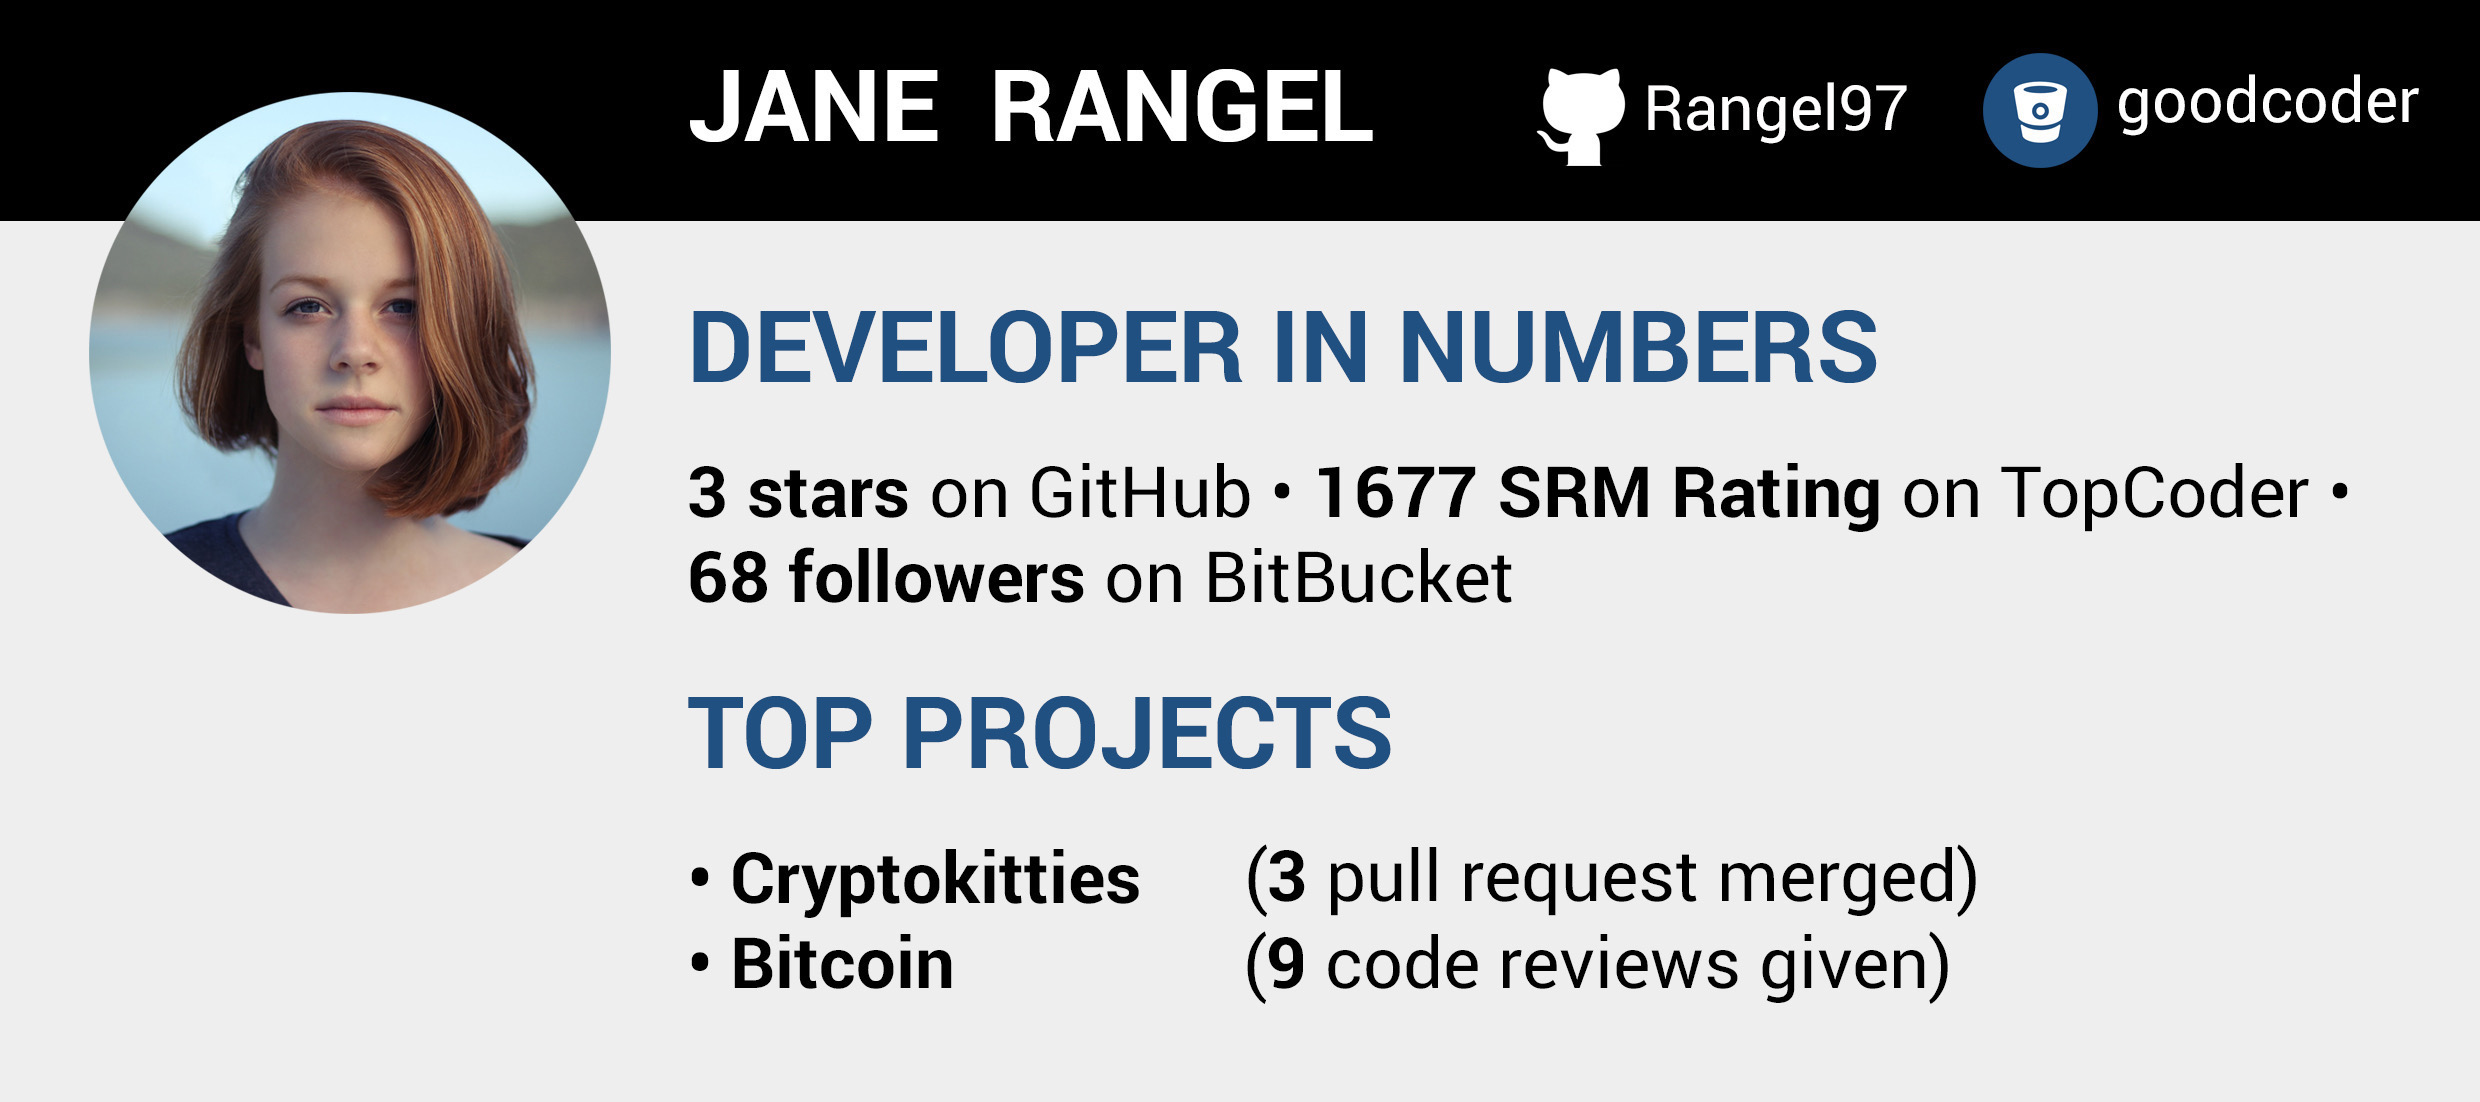
\includegraphics[width=\columnwidth]{devid/resources/devid_smaller.jpeg}
	\caption{An impression of a DevID portfolio. These infographics can be automatically generated and customized based on records in a DevID portfolio.}
	\label{fig:devid}
\end{figure}

We then build a decentralized crowdsourcing marketplace for the development of dApps, named \emph{dAppCoder}.
Our platform enables clients to post projects and developers to find projects that match with their expertise.
All payments are conducted directly between clients and developers, sidestepping the need a trusted intermediary for payment processing and commissions.
%Within the context of \Dappcoder, DevID records are used by the client to filter prospective developers and to make educated decisions on who to hire for a particular job.
We believe that our single, public, and open crowdsourcing market has the potential to be more efficient compared to a centralized solution with fragmentation and lock-in effects.

The main contribution of this work is tri-fold:
\begin{itemize}
	\item We first present \emph{DevID}, a unified portfolio for dApp developers (Section~\ref{sec:devid_architecture}). DevID stores records associated with a developer, e.g., GitHub projects, on a scalable blockchain ledger with high scalability and low overhead.
	\item We then present \emph{dAppCoder}, a decentralized crowdsourcing market for the development of dApps (Section~\ref{sec:dappcoder}).
	\item Finally, we discuss our \emph{deployment trial} of DevID and dAppCoder with a small group of users, which demonstrates the practicality of our work (Section~\ref{sec:experiments}).
\end{itemize}

\section{Problem Description}
\label{sec:problem_description}
We identify challenges in two directions.
First, we wish to create a developer portfolio that gives an accurate impression of their capabilities and expertise.
Second, we aim to build a decentralized crowdsourcing marketplace for the development of dApps.
We elaborate on the challenges associated with each contribution.

\textbf{Developer portfolios.}
We list three main requirements for this portfolio.
First, we require that developers are able to \emph{import existing data} from other platforms into their portfolio.
This streamlines the bootstrapping process of a portfolio with relevant records since a developer is likely to use multiple platforms to store and work on their projects (e.g., GitHub and LinkedIn).
However, not all platforms have built-in tools to easily export personal data to another ecosystem.
Additionally, it is key to ensure that data being imported actually belongs to the user importing it, preventing a malicious user from impersonating someone else.
We consider the import process of personal data an essential requirement to ensure trustworthy portfolios.

Second, we require portfolio records to be tamper-proof.
Specifically, we want to avoid the situation where a developer temporarily inflates its portfolio when applying for a particular project.
Modifications to a DevID portfolio should be transparent and traceable.

Third, we require our developer portfolio to be \emph{independent of any trusted intermediary}.
Specifically, in the context of our work this means that the data itself is not managed by a trusted authority but instead by the operating user itself.
Blockchain technology is increasingly being used as middleware for building decentralized applications without centralized authority.
For example, platforms like Ethereum and EOS enable developers to write and deploy smart contracts, self-executing code that enforces agreements between two or more parties~\cite{szabo1997formalizing}.
However, most blockchain fabrics are not suitable for large-scale storage of portfolio records, or for data storage in general due to their limited throughput and, for some platforms, prohibitively high transaction fees~\cite{eberhardt2017or}.
Therefore, we prefer an alternative, more lightweight solution to store portfolio records.

\textbf{Crowdsourcing Market.}
Similar to the requirements of our developer portfolios, a key requirement for our crowdsourcing market is that there is no intermediary responsible for creating and managing projects, and for matching clients with developers.
Instead, all information should be managed in a decentralized manner, namely by peers in the network themselves.

Given these requirements, the research question of this work is as follows:
\textit{How can we build a decentralized crowdsourcing platform for the development of dApps?}
\begin{figure}[t!]
	\centering
	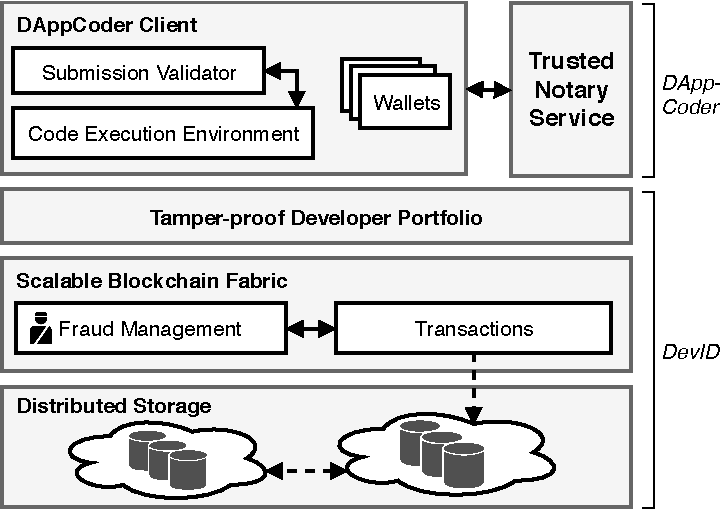
\includegraphics[width=.7\linewidth]{devid/resources/architecture.pdf}
	\caption{The architecture of DevID and dAppCoder.}
	\label{fig:system_architecture}
\end{figure}

\section{DevID: Unified Portfolios for Software Developers}
\label{sec:devid_architecture}
We now present our unified developer portfolio, named \emph{DevID}.
The architecture is given in Figure \ref{fig:system_architecture}.
This figure also includes the architecture of dAppCoder, our platform to crowdsource the development of decentralized applications.
dAppCoder itself is discussed later in Section~\ref{sec:dappcoder}.

\subsection{Record Types}
\label{subsec:record_types}
DevID distinguishes between the following seven record types:

\textbf{Personal information.}
This record contains personal information associated with the developer, for example, a full name, a profile picture, an email address, or a GitHub username.

\textbf{Statistics.}
Statistics are quantifiable and verifiable numbers that represent a specific developer metric.
For example, these records could represent developer statistics like the number of years of programming experience, or the total number of code reviews given.
A visualization of these records is shown in Figure~\ref{fig:devid} under the section \enquote{Developer in Numbers}.

\textbf{Projects.}
Developers can add projects to their DevID portfolio, for example, open-source software projects where the developer has contributed to.
In Figure~\ref{fig:devid}, this information is displayed under the section \enquote{Top Projects}.
Optionally, a reference to a project can be added to a DevID portfolio, such as a link to a GitHub repository or to the hash of a particular commit.

\textbf{Skills.}
Developers can add skills to their DevID portfolio.
We consider the ability to highlight proficiency in specific programming languages and familiarity with blockchain platforms an essential feature of a developer portfolio.
It aids programmers in finding projects that match their expertise, and it enables clients to find developers that fit their projects best.
For instance, applications that have access to DevID portfolios can filter available developers on one or multiple skills, therefore reducing search frictions.
%Figure~\ref{fig:devid} shows two skills under the section \enquote{Programming Skills}.

\textbf{Endorsements.}
Another record type we define is endorsements.
Developers can endorse other developers (e.g., by writing a letter of recommendation) or endorse specific skills of others.
Skills and endorsements can also be imported from other platforms like LinkedIn, which is discussed in the next section.

\textbf{Import.}
Developers are able to import data from other sources into their DevID portfolio.
When performing an import action, a record with this type is created, containing specifications on the import source, and the imported data elements.
Other records can reference the import record, for example, to signify that a particular skill endorsement has been imported from LinkedIn.
We describe record specifications and references between these records in Section~\ref{subsec:devid_record_specs}.

\textbf{Wallets.}
Finally, developers can add the specifications of wallets to their DevID portfolio, for example, the address of their Bitcoin wallet.
We envision that DevID portfolios will be utilized when developers are looking for work, and embedding payment addresses directly in the portfolio speeds up the payout process when a developer has performed work.
It also enables developers to quickly receive donations as compensation for community work.

We believe that the above record types are sufficient for developers to build a basic portfolio.
The implementation of DevID is flexible and allows system designers to add additional record types after deployment.

\subsection{Unifying Developer Data}
\label{subsec:unifying_data}
We now discuss how to import developer data from multiple platforms in a DevID portfolio and how to verify the correctness of the imported data.

\textbf{Importing developer data.}
DevID allows developers to import relevant information from different platforms into their portfolio.
For example, they can import data from LinkedIn (e.g., skills or past projects) or from GitHub (e.g., the number of followers and code contributions).
Importing can be done by querying their public interfaces (APIs) and request the relevant data, if this is supported by the platform.
To store the data in the portfolio, one can either add a reference to the (external) data or copy the data assets into the portfolio.
To reduce dependency on third-party services, we choose to copy the data and store it within a portfolio record.

\textbf{Verifying developer data.}
As discussed in Section~\ref{sec:problem_description}, it is essential to ensure that imported data actually belongs to the developer importing it.
We propose two solutions to achieve trustworthy importation of data: \textit{challenges} and \textit{TLS auditing}.

The first solution is to pose a challenge where the developer importing the data, proves that they have control over this data.
For example, when importing data from GitHub, we can require a public identifier (e.g., a public key) of the developer to be part of the \enquote{bio} profile field.
This information can then be verified for correctness by other users who query the public GitHub API.
We call users who verify data \emph{witnesses}.
While this is a basic mechanism to ensure the accuracy of imported data, it heavily depends on the availability of a public API.

The second solution is TLS auditing~\cite{tlsnotary2014whitepaper}.
The key idea is to proxy a TLS connection through a random witness, which then verifies and signs the data after the TLS connection terminates.
When the TLS session finishes, the client gives the witness the private key used to decrypt HTTPS responses from the web service.
Note that this way the witness is not able to decrypt the request made to the web service, which likely includes credentials or access tokens.
The role of a witness can either be fulfilled by other entities in the network, or by a trusted notary service.
Depending on the significance of data being imported, multiple witnesses can be used for this.
Compared to challenges, TLS auditing works when access to a public API is absent but is more advanced.
Our lab has implemented an advanced TLS auditing mechanism, which is currently under a security audit.

\subsection{Verified Identities}
\label{subsec:strong_identities}
In DevID, users are identified by a self-generated public key and digitally sign portfolio records with their private key.
This allows for the Sybil Attack, the situation where a real-world persona can operate many different DevID portfolios~\cite{douceur2002sybil}.
To address this situation, developers can verify their digital identity.
A verified identity is uniquely linked to a real-world entity.
Software built on DevID can give preferential treatment to developers that have verified their identity.
For example, an application can ignore endorsements that are given by developers with an unverified identity, and clients can only consider developers with a verified identity for a particular project.
The user interface of \Dappcoder{} highlights verified users with a special badge.
Identity verification can be done with an attestation provided by a trusted third party like the government or a notary.
Strong, long-lived identities in DevID is comparable with account validation that many centralized platforms use (e.g., the verification of a phone number).
Since misbehaviour can be traced back to the real-world persona, it also raises the barrier for users to collude with each other, e.g., tit-for-tat behaviour when creating endorsements.

\begin{figure*}[t!]
	\centering
	\begin{subfigure}[t]{.5\textwidth}
		\centering
		\captionsetup{width=.9\linewidth}
		\raisebox{4mm}{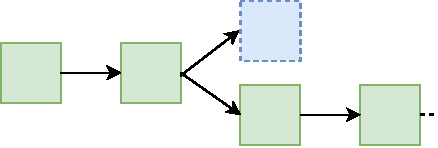
\includegraphics[width=.9\linewidth]{devid/resources/blockchain_single}}
		\caption{Linear ledger (Ethereum).}
		\label{fig:blockchain_single}
	\end{subfigure}%
	\begin{subfigure}[t]{.5\textwidth}
		\centering
		\captionsetup{width=.9\linewidth}
		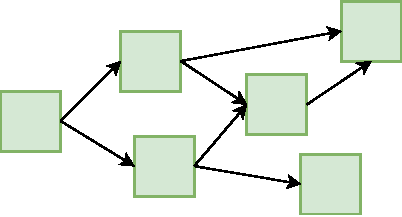
\includegraphics[width=.9\linewidth]{devid/resources/blockchain_dag}
		\caption{DAG ledger (IOTA).}
		\label{fig:blockchain_dag}
	\end{subfigure}\vspace{0.5cm}
	\begin{subfigure}[t]{.5\textwidth}
		\centering
		\captionsetup{width=.9\linewidth}
		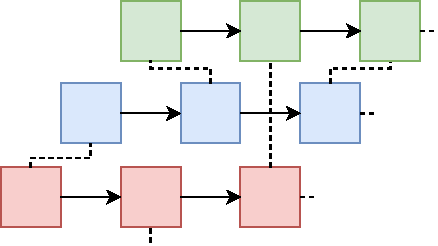
\includegraphics[width=\linewidth]{devid/resources/blockchain_pairwise}
		\caption{Pairwise ledger (Nano).}
		\label{fig:blockchain_pairwise}
	\end{subfigure}%
	\caption{Three different structures of distributed blockchain ledgers. Each arrow points to the subsequent block in the chain. The dotted block in (a) indicates a fork.}
	\label{fig:blockchain_structures}
\end{figure*}

\subsection{Efficient Blockchain Storage}
\label{subsec:scalable_blockchain}
DevID requires an data structure that can store tamper-proof and accurate data records.
Blockchain technology is gaining traction as platform to store verified transactions.
We now discuss three common blockchain organizations, visualised in Figure~\ref{fig:blockchain_structures}, and analyse their trade-offs in the context of our work.

\textbf{Linear ledger.} Figure~\ref{fig:blockchain_single} shows a linear blockchain ledger, which is used by platforms such as Bitcoin~\cite{nakamoto2008bitcoin} and Ethereum~\cite{wood2014ethereum}.
This ledger consists of multiple blocks and each block contains transactions.
Every block, except for the first one, points back to the prior block in the ledger through a hash pointer.
Usually, this type of ledger is safeguarded by a consensus mechanism where at least a majority of users continuously reach agreement on the exact sequence of transactions.
A network-wide consensus mechanism like Proof-of-Work or Proof-of-Stake prevents the situation where a malicious user intentionally creates a fork of their chain to override prior transactions~\cite{vukolic2015quest}.
While linear ledgers providing a relatively high level of security, the transaction throughput of these ledgers is often not sufficient to facilitate record creation and modification by millions of users.
This motivates us to consider different types of blockchain for portfolio storage.

\textbf{DAG ledger.} Another blockchain structure is the Directed Acyclic Graph (DAG) ledger, where each block can be referenced by multiple other blocks.
This ledger structure, shown in Figure~\ref{fig:blockchain_dag}, is adopted by blockchain platforms like IOTA and Dagcoin~\cite{popov2018tangle}~\cite{lerner2015dagcoin}.
IOTA is optimized for micro-payments within Internet-of-Things, and Dagcoin advertises itself as data storage for arbitrary data (e.g., documents or ownership records).
Since these ledgers allow for different consensus mechanisms, transaction throughput is often superior compared to that of linear ledgers.
However, they usually have differing security guarantees.
While these ledger structures are more suitable for data storage, we consider current implementations unfit for developer portfolios.
The reason is that they either rely on a centralized coordinator (IOTA) or a fixed group of witness nodes (Dagcoin).
Instead, our goal is to devise a portfolio infrastructure without any authority with leveraged permission.

\textbf{Pairwise Ledger.} A third blockchain structure we consider is the pairwise distributed ledger.
The key property of this ledger, given in Figure~\ref{fig:blockchain_pairwise}, is that each user maintains and grows their individual chain with transactions.
Each block holds exactly one transaction and optionally contains a (hash) pointer to a transaction in the individual chain of another user.
Blockchain fabrics like R3 Corda~\cite{brown2017introducing}, Nano~\cite{lemahieu2017raiblocks}, and TrustChain~\cite{otte2017trustchain}, use pairwise ledgers as their underlying data structure.
These platforms address the double-spending attack either by a trusted notary (Corda), a weighted voting system (Nano) or by guaranteed eventual consistency (TrustChain).
In general, they can provide superior scalability compared to linear ledgers as used by Bitcoin and Ethereum.

We believe that the pairwise distributed ledger is a suitable data structure to store portfolio records as transactions.\footnote{The work describing TrustChain considers a personal ledger as a collection of \emph{records}. To avoid semantic overload, we use the term transaction to refer to a TrustChain record.}
Compared to linear and DAG ledgers, all data of a portfolio owner is local to their own personal ledger and maintained by themselves.
Specifically, we choose to build DevID and subsequently \Dappcoder{} (see Section~\ref{sec:dappcoder}), using the TrustChain data structure.
TrustChain, first introduced by Otte et al.~\cite{otte2017trustchain}, is a lightweight distributed ledger where each user maintains a personal ledger.
To detect malicious behaviour, in particularly the forking of a personal ledger, users continuously request random transactions from other users and share their transactions with other users upon request.
The consistency of incoming transactions is checked against known transactions, and illegitimate modifications of the personal ledger can quickly be revealed by the collective effort of users in the network.

TrustChain has four particular advantages that align with developer portfolios.
First, TrustChain enables selective queries of data stored on the chains of other members, without the need for full data replication across the network.
Second, TrustChain is particularly designed for the tamper-proof accounting of generic data elements.
Third, while TrustChain is primarily built around bilateral transactions, this ledger architecture also supports unilateral transactions.
Unilateral transactions are particularly helpful when storing content that is not related to other users, e.g., when a developer includes a project in its portfolio.
Finally, TrustChain is already used as transaction fabric within a self-sovereign, decentralized identity system, described in the work of Stokkink et al~\cite{stokkink2018deployment}.
Availability of a self-sovereign identity system aligns with our requirement for strong, long-lived identities (see Section~\ref{subsec:strong_identities}).
TrustChain, however, does provide less consistency guarantees but we believe that this does not pose a barrier for DevID (depending on the system parameters and network size, malicious behaviour can usually be detected within seconds).

\begin{figure}[t!]
	\centering
	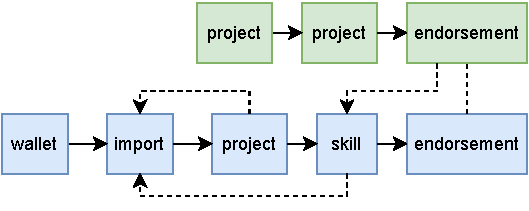
\includegraphics[width=.8\linewidth]{devid/resources/trustchain_devid.pdf}
	\caption{Example of DevID records and links between them on two TrustChain personal ledgers (coloured differently). Solid arrows indicate hash references between transactions whereas dashed arrows indicate application-specific references included in the transaction payload.}
	\label{fig:devid_trustchain}
\end{figure}

\subsection{DevID records and TrustChain}
\label{subsec:devid_record_specs}
TrustChain enables users to issue transactions with an application-specific payload.
These transactions are appended to the personal ledger of the operating peer and shared with others.
TrustChain also enables system designers to specify validity rules for different transaction types.
A TrustChain transaction has a \texttt{type} field, which we fix as the record types discussed in Section~\ref{subsec:record_types} with \texttt{devid\_} as prefix.
The transaction type is used by participating users to distinguish between different applications and to conduct application-specific validation of incoming transactions (since different applications operate on the same the TrustChain infrastructure).
%TrustChain is built around bilateral transactions but also support unilateral transactions that do not require the agreement of other users.
The transactions containing records associated with projects, skills, import actions, and wallet information are unilateral.
Endorsements are implemented as bilateral transactions since they involve an interaction between two users.
However, endorsements do not strictly require a counter-transaction from the user being endorsed.
An endorsement contains a reference to the transactions containing the skills being endorsed.

Figure~\ref{fig:devid_trustchain} shows how DevID records are mapped on the TrustChain data structure.
The figure shows (a part of) the personal ledger and TrustChain transactions of two different users $ a $ and $ b $, in green and blue colours, respectively.
User $ a $ added two projects to its portfolio and provided an endorsement to user $ b $.
User $ b $ added information about a particular wallet to its portfolio and subsequently imported data from an external source.
This import action added a single project and skill to the portfolio of user $ b $.
The transactions associated with the project and skill reference the transaction containing the import details.

Users joining the network continuously request TrustChain transactions from other users and consequently build up knowledge of the DevID portfolios of others.
Upon receiving TrustChain transactions, users will invoke an application-specific validation process that depends on the transaction type.
This involves a check whether the transaction payload is well-formatted and contains all expected fields.
Some transaction types require more extensive validation, for example, validating \texttt{import} transactions.
Since there are no guarantees on the order in which TrustChain records arrive, the validation of transactions that are linked to an import action (e.g., projects) is delayed until the \texttt{import} transaction has been received and verified.

\subsection{Storing Large Data Assets}
While pairwise distributed ledgers are suitable for storing small portfolio records, they are not suitable for storing arbitrary large data assets.
Such data assets can include source code, documentation, videos, and reviews.
To overcome this, we leverage off-chain distributed storage solution that offers data immutability and scalability.
Figure~\ref{fig:system_architecture} includes this distributed storage, which comprises the lowest layer in our architecture.

We wish to avoid data storage by a trusted operator.
Suitable distributed storage solutions for our work are a Distributed Hash Table (DHT) like Kademlia, a BitTorrent swarm or the InterPlanetary File System (IPFS)~\cite{maymounkov2002kademlia,cohen2008bittorrent,benet2014ipfs}.
These solutions enable users to store large data assets, without involvement of a trusted third party.
Large data is inserted in the distributed storage back-end, and a reference to the data (i.e., a content hash) is included in the on-chain transaction.
DevID (and DAppCoder) users can store their data at different \emph{providers}.
DevID portfolio records with external data assets attached include the provider identifier (e.g., \enquote{\texttt{IPFS}}) and a pointer to the data (e.g., an IPFS content hash).

\section{dAppCoder: Crowdsourcing Development of Decentralized Applications}
\label{sec:dappcoder}
By extending the DevID portfolio architecture, we build a crowdsourcing marketplace, named \emph{dAppCoder}, for the development of decentralized applications.
Running completely without centralized servers, \Dappcoder{} enables clients to propose projects and to find developers qualified to work on their projects.
The process of finding developers is streamlined by direct integration of DevID portfolios, therefore reducing search frictions.
dApp developers can choose to work on projects that match their skill set.
\Dappcoder{} also provides primitives for project management and financial compensation for developers.
With a direct integration with DevID portfolios, developers can work on their reputation by participating in dAppCoder projects.
The architecture of \Dappcoder{} is presented in the upper layer of Figure~\ref{fig:system_architecture}.
We now elaborate on the main functionalities of \Dappcoder{}.

\begin{lstlisting}[language=json,firstnumber=1,float=t,caption=A project offered in DAppCoder (in JSON format).,label=lst:devid_project]
{
	"title": "An Ethereum-based Art Marketplace",
	"description": {
		"provider": "IPFS",
		"uri": "..."
	},
	"requirements": {
		"provider": "IPFS",
		"uri": "..."
	},
	"deadline": "20-09-2021",
	"required_skills": ["Solidity", "Ethereum"],
	"compensation": {
		"height": "...",
		"deposit": "...",
	},
	"assets": [{
		"description": "example art objects",
		"provider": "IPFS",
		"uri": "..."
	}]
}
\end{lstlisting}

\subsection{Creating and Managing Projects}
Clients that want their idea realized (e.g., the implementation of a particular smart contract) can offer a new project in \Dappcoder{}.
Creating a new project requires the client to specify various fields, as exemplified in Listing~\ref{lst:devid_project}.
Each project includes a title, a description, a list with technical requirements for the final deliverable, a deadline (optional), a list of required skills needed to successfully complete the project, the height of the compensation (if any). and an optional list of assets provided by the client.
Since the project description, requirements, and assets can become large, these assets are stored off-chain and a reference to these assets is included in the transaction.
This reference contains a \texttt{provider} and \texttt{uri} field.
To publish a project, a TrustChain transaction with type \texttt{dappcoder\_project} containing all project information is constructed, appended to the personal ledger of the project creator, and disseminated in the network.
Clients can publish projects that concern both open-source deliverables (e.g., a publicly deployed Ethereum smart contract) and closed-source deliverables (e.g., a smart contract deployed in a private blockchain).
\Dappcoder{} supports direct payouts between clients and developers using cryptocurrency.
This avoids the need for trusted intermediaries for payment processing.
%For each new project, the client generates a \textit{project keypair}, which consists of a public and private key.
%These keys are used when releasing the submissions for a project, which is discussed in Section~\ref{subsec:create_submissions}.

%A key feature of dAppCoder is built-in support for financial compensation of a developer that has performed some work on a project.
%Prior to publishing a new project, the client determines the height of the reward, if there is any, and transfers these funds to a \textit{Trusted Notary Service} (shown in Figure~\ref{fig:system_architecture}).
%This trusted notary service manages developer payouts and is external to the DevID and DAppCoder ecosystem.
%The trusted notary can either be a centralized authority or an (Ethereum) smart contract that interacts with the dAppCoder application through oracles.
%The compensation, put into escrow, addresses the situation when a dispute arises between client and developer and the client refuses to pay the developer for their work.
%This dispute is then mediated by the trusted notary, whether or not with the involvement of the developer and client.
%When receiving a TrustChain transaction containing a project with a compensation, the software automatically checks whether the deposit is valid and confirmed by the trusted notary service.

As shown in Figure~\ref{fig:devid_project}, a dAppCoder project can be in one of the five following stages: \emph{created}, \emph{implementing}, \emph{testing}, \emph{finished} or \emph{cancelled}.
After a project has been created, developers can indicate their interest to work on a preferred project by creating and sharing a unilateral \texttt{dappcoder\_project\_interest} transaction.
A client is still able to cancel projects that have not advanced to the implementation stage.
If many developers have indicated their interest to work on a particular project, the client can filter developers, for example, based on the information in their DevID portfolios.
A project is updated using a \texttt{dappcoder\_project\_update} transaction created by the project creator that transitions the project to a different stage.
The \Dappcoder{} software has built-in validation rules that assess whether a project transaction is valid.
For example, a project cannot transition from the \emph{cancelled} to \emph{created} stage and transactions containing such a transaction are ignored.

During the implementation stage, assigned developers work on implementing the project deliverables.
When the implementation is complete, the project enters the \emph{testing} stage.
Testing is a crucial requirement for the development of secure decentralized applications that often evolve around value transfer or business-critical operations.
A single bug has the potential to bring down an ecosystem that manages billions worths of assets, as demonstrated by the DAO hack in 2016~\cite{dhillon2017dao}.
This testing might be performed by the developers that worked on the project deliverables during the implementation stage, or by other developers.
If the testing stage reveals that more work is needed on the project deliverable, the project can transition to the \emph{implementing} stage again.
This is ultimately determined by the client.
When the deliverable is satisfactory, the client indicates that the project is finished and conducts payments to the involved developers.

\begin{figure*}[t!]
	\centering
	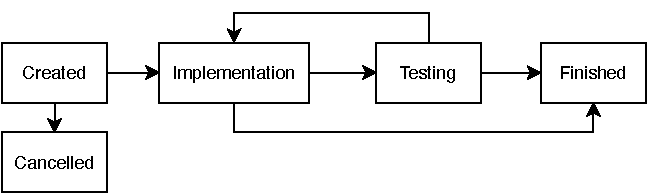
\includegraphics[width=0.8\textwidth]{devid/resources/devid_project.pdf}
	\caption{The different stages of a project in dAppCoder, and their transitions.}
	\label{fig:devid_project}
\end{figure*}

\subsection{Finding Projects and Publishing Deliverables}
\label{subsec:create_submissions}
Developers looking for work can browse through the list of open projects, or filter them based on the skills they have added to their DevID portfolio.
When a developer has found an interesting project, they indicate their interest to work on the project.
This work starts when the client assigned the interested developer to the project and when the project transitions to the implementation phase.
If the source code of the project can be made public, a developer may create a \texttt{dappcoder\_deliverable} transaction that includes a pointer to the work done.
This pointer, for example, can refer to a GitHub repository.
Such a transaction also links to the project associated with the submission.

%\subsection{Testing Submissions}
%\label{subsec:review_submissions}
%After the submission deadline passed, all submissions should be tested by other developers.
%For simplicity, we assume that the client selects appropriate testers for submissions, based on their expertise (indicated by their DevID portfolio) and the total number of submissions tested in the past.
%To incentivize developers to test submissions, testing activities will be prominently displayed on their DevID portfolio.
%The testing phase consists of two phases, where tests are written and verified.
%To avoid collusion between developers, we require that individuals who have created a submission, written tests, and verified these tests, are not affiliated.

%\textbf{Writing tests:}
%First, testers write tests to verify the correctness of a submission.
%These tests can be used to expose critical vulnerabilities or programming errors in business-critical code.
%If a tester found such an error, they can mark the submission for exclusion and should provide a test that highlights it.

%Besides writing tests, each tester grades the submission based on compliance to the specifications.
%The given score can range from "very low" (-2), "low" (-1), "neutral" (0), "sufficient" (1) or "high" (2).

%\textbf{Verifying tests:}
%Second, developers inspect the tests, written by testers in the previous phase.
%In particular, thoroughness and completeness of the tests written by a specific tester will be graded by giving a similar score as in the previous phase.

\subsection{Paying Out Developers}
\label{subsec:dappcoder_payout}
dAppCoder has built-in tools to directly payout developers that worked on a paid project.
The time at which these payouts take place should be decided between the developer and client using an out-of-band communication channel.
For example, a developer can request to be partially compensated up-front.
We envision that all payouts in dAppCoder proceed using cryptocurrencies and are public.
A developer can signify a payout by creating a \texttt{dappcoder\_payout} transaction, containing a reference to the cryptocurrency transaction associated with the payout (e.g., the hash of a Bitcoin transaction).
By verifying the source and destination wallet addresses of the payout, other users can determine whether a client correctly compensated a developer.
Unreliable clients that have no valid payout associated with a finished and paid project will be flagged in the application and can be avoided by developers.

\section{Implementation and Deployment Trial}
\label{sec:experiments}
Next, we elaborate on the implementation of both the DevID portfolios and the dAppCoder application.
We also discuss our deployment trial and present preliminary results.

\begin{figure*}[t!]
	\centering
	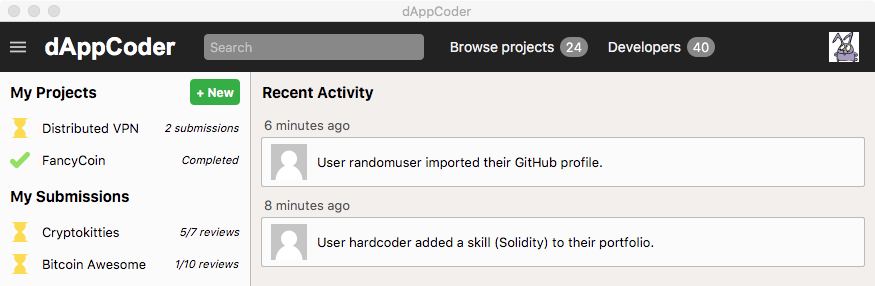
\includegraphics[width=0.99\textwidth]{devid/resources/gui_smaller.png}
	\caption{The user interface of DAppCoder, our application to crowdsource the development of decentralized applications.}
	\label{fig:dappcoder}
\end{figure*}

\subsection{Implementation}
We have implemented both DevID and dAppCoder in the Python programming language.
Our implementation consists of all components shown in Figure~\ref{fig:system_architecture}.
The graphical user interface of dAppCoder is visualized in Figure~\ref{fig:dappcoder} and is implemented with the Qt5 library.
It communicates with the back-end over a RESTful API.
The open source implementations of both DevID and dAppCoder are available online.\footnote{See \url{https://github.com/tribler/dappcoder}.}

We build DevID, and by extension dAppCoder, on the TrustChain ledger introduced by Otte et al~\cite{otte2017trustchain}.
We use the InterPlanetary File System (IPFS) to store large data assets like project specifications, submissions and code reviews.
Users can import statistics from their GitHub profile using the challenge mechanism described in Section~\ref{subsec:unifying_data}.

\subsection{Deployment Trial}
To assess the feasibility of dAppCoder and to get insight into the efficiency of the TrustChain ledger, we conduct a deployment trial.
We present the trial setup and results.

\textbf{Setup:}
For our trial, we recruited 15 participants among local staff and students of our faculty.
Each participant interacts with the dAppCoder application for around 15 minutes and during this time, participants were free to use the application as they see fit.
To bootstrap the application, we initiated dAppCoder with five unpaid projects ourselves.
Two of these projects asked developers to resolve one or more bugs in a piece of Python code.
The other three projects asked the developer to implement a small application.
Since only a fraction of our users is familiar with the development of decentralized applications, we accepted submissions in other programming languages during our trial, like Java.
We collected data and observed the growth of the distributed ledger over a period of five working days.


\begin{figure}[t!]
	\centering
	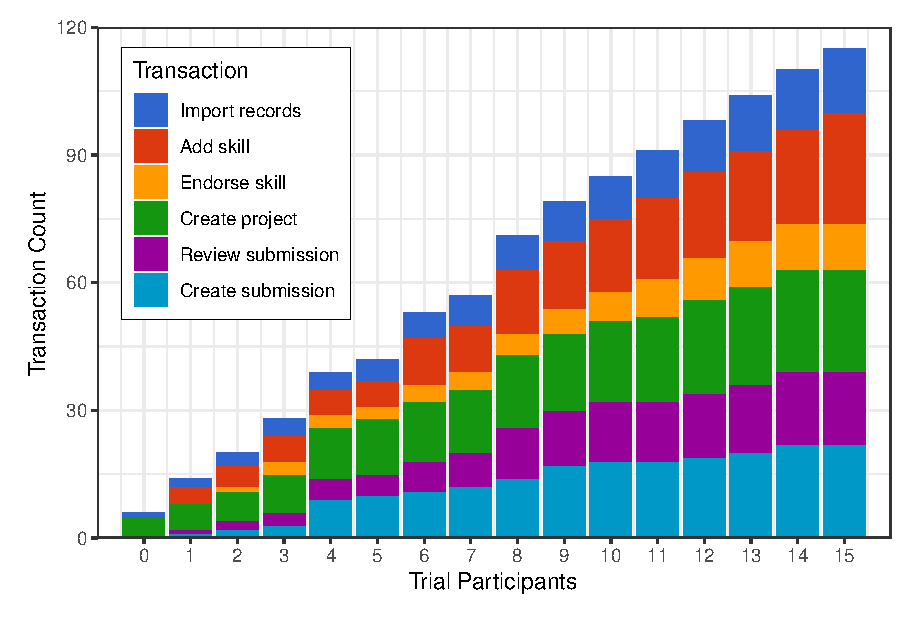
\includegraphics[width=.75\columnwidth]{devid/resources/experiment/experiment_1_unit.eps}
	\caption{Results from our deployment trial.}
	\label{fig:experiment_graph}
\end{figure}

\textbf{Results:}
Figure~\ref{fig:experiment_graph} shows the growth of the TrustChain ledger, in terms of transactions, when more participants join the trial.
Each entry on the horizontal axis represents the state of the ledger after a participant was introduced, and the vertical axis shows the transaction count for the six different types of transactions.
When more participants join, the distribution of transaction types on the ledger changes slightly.
We observe that the growth of projects over time decreases, and users focus more on creating submissions and reviews.
We remark that the version of \Dappcoder{} subjected to the user trial oriented around competition-based crowdsourcing and participants are able to review the submissions of others.
Another observation is that the number of skills added by each developer grows rapidly, but the growth of endorsements stays behind.

At the end of our deployment trial, the average transaction size in serialized form is 0.6 kB.
The total size of all transactions stored on the distributed ledger is 65.4 kB.
Each personal ledger stores on average 7.2 transactions, with an average size of 4.1 kB.
In comparison, when using a linear ledger like Bitcoin, each user is required to store the entire global ledger or parts of it.  
The time required to append new transactions to the TrustChain ledger is in the range of milliseconds and not of influence on the user experience.
The initial results of the trial look promising, and we are ready for further evaluation of \Dappcoder{} and DevID portfolios. 

\section{Related Work}
We are the first to build a tamper-proof and unified developer portfolio, to the best of our knowledge.
Already in 1995, research has been conducted, that explores the advantages of online electronic portfolios over traditional resumes, particularly within an educational environment~\cite{riggsby1995electronic,barrett2000electronic}.
The emergence of the open source software paradigm enabled developers to use code contributions as proof of verifiable technical expertise and to build an online reputation~\cite{riehle2015open}.
The work of Cai et al. explores how this data can be used to construct a theoretical reputation model, and what metrics would be best suited for this~\cite{cai2016reputation}.
Other work is focused on visualization tools to highlight contributions of the individual developer on platforms like GitHub or StackOverflow~\cite{jaruchotrattanasakul2016open,saxena2017know,chen2016supporting}.
Their research is primarily focused on the design and evaluation of models to represent the technical skills, based on data from open source projects.
The focus of this work is on combining records from different platforms and presenting them in a unified portfolio.

The evolution of crowdsourcing and the benefits are well-studied topics with an extensive literature corpus~\cite{latoza2016crowdsourcing}.
TopCoder Inc. is an example of a crowdsourcing platform where clients can outsource software contributions to developers in a competition-based environment~\cite{lakhani2010topcoder}.
In 2017, Li et al. introduced CrowdBC, a decentralized blockchain-based framework for crowdsourcing~\cite{li2017crowdbc}.
CrowdBC is a platform to crowdsource generic micro-tasks and is not suitable to crowdsource development of decentralized applications.
Lu et al. devised a privacy-preserving crowdsourcing mechanism on top of an open blockchain~\cite{lu2018zebralancer}.
Zou et al. present a consensus protocol that is suitable for crowdsourcing tasks~\cite{zou2018proof}.
The protocol selects transaction validators and addresses unfaithful behaviour when participating in the system.
Buccafurri et al. introduce TweetChain and show how to build a crowdsourcing application which stores all information on Twitter timelines~\cite{buccafurri2017tweetchain}.
TweetChain is comparable with personal ledgers in TrustChain but depends on a central authority for dissemination and storage of data (Twitter).
In comparison to most of the research performed on blockchain-based crowdsourcing, this work focuses on a specific use-case, namely crowdsourcing the development of business-critical applications.

\section{Conclusions}
We have presented dAppCoder, a decentralized crowdsourcing platform for the development of decentralized applications.
As a first step, we build DevID, a unified portfolio for software developers.
DevID addresses the fragmentation and lock-in of developer data across different platforms with a mechanism to import data from third-party services.
By building upon an existing scalable ledger, DevID is capable of storing tamper-proof records and does not depend on any trusted party.
Portfolio records are fully managed by developers themselves.
Our application, dAppCoder, matches clients and reputable developers.
With a deployment trial, we have demonstrated that dAppCoder is feasible.

Future work is focused on a large-scale deployment of dAppCoder and better support for specific bug bounties.
We envision the integration of multiple cryptocurrencies and external data providers.
Using our TLS auditing mechanism, we plan to expand DevID with the ability to import data elements from other platforms, in particular, LinkedIn and StackOverflow.
Finally, we aim to explore the use of DevID within other domains besides crowdsourcing.